% !TeX encoding = UTF-8
% !TeX spellcheck = fr_FR


\chapter{Conceptualisation et analyse de faisabilité}
\label{s:concpt_anals}


% !TeX encoding = UTF-8
% !TeX spellcheck = fr_FR


\definecolor{couleurbackintr}{HTML}{7F00FF}
\definecolor{couleurtextintr}{HTML}{FFFFFF}
\definecolor{couleurbackfonc}{HTML}{C780FF}
\definecolor{couleurtext}{HTML}{000000}
\definecolor{couleurbackextr}{HTML}{DDB3FF}

\newcommand{\multiliens}[2]{\foreach \noeud in {#1} {\draw[<-] (#2.west) -| ++(-1em,0em) |- (\noeud.east);}}
\newcommand{\lienhorz}[2]{\draw[->] (#1.east) -- (#2.west);}
\newcommand{\lienvtht}[2]{\draw[->] (#1.north) -- (#2.south);}
\newcommand{\lienvtbs}[2]{\draw[->] (#1.south) -- (#2.north);}


\begin{figure}[htp]
	\centering
	\tikzset{
		basic/.style={draw, rounded corners=2pt, thick, text width=8em, align=flush center, text=couleurtext, node distance=2em},
		intrant/.style={basic, fill=couleurbackintr, text=couleurtextintr},
		fonction/.style={basic, fill=couleurbackfonc},
		extrant/.style={basic, fill=couleurbackextr}
	}
	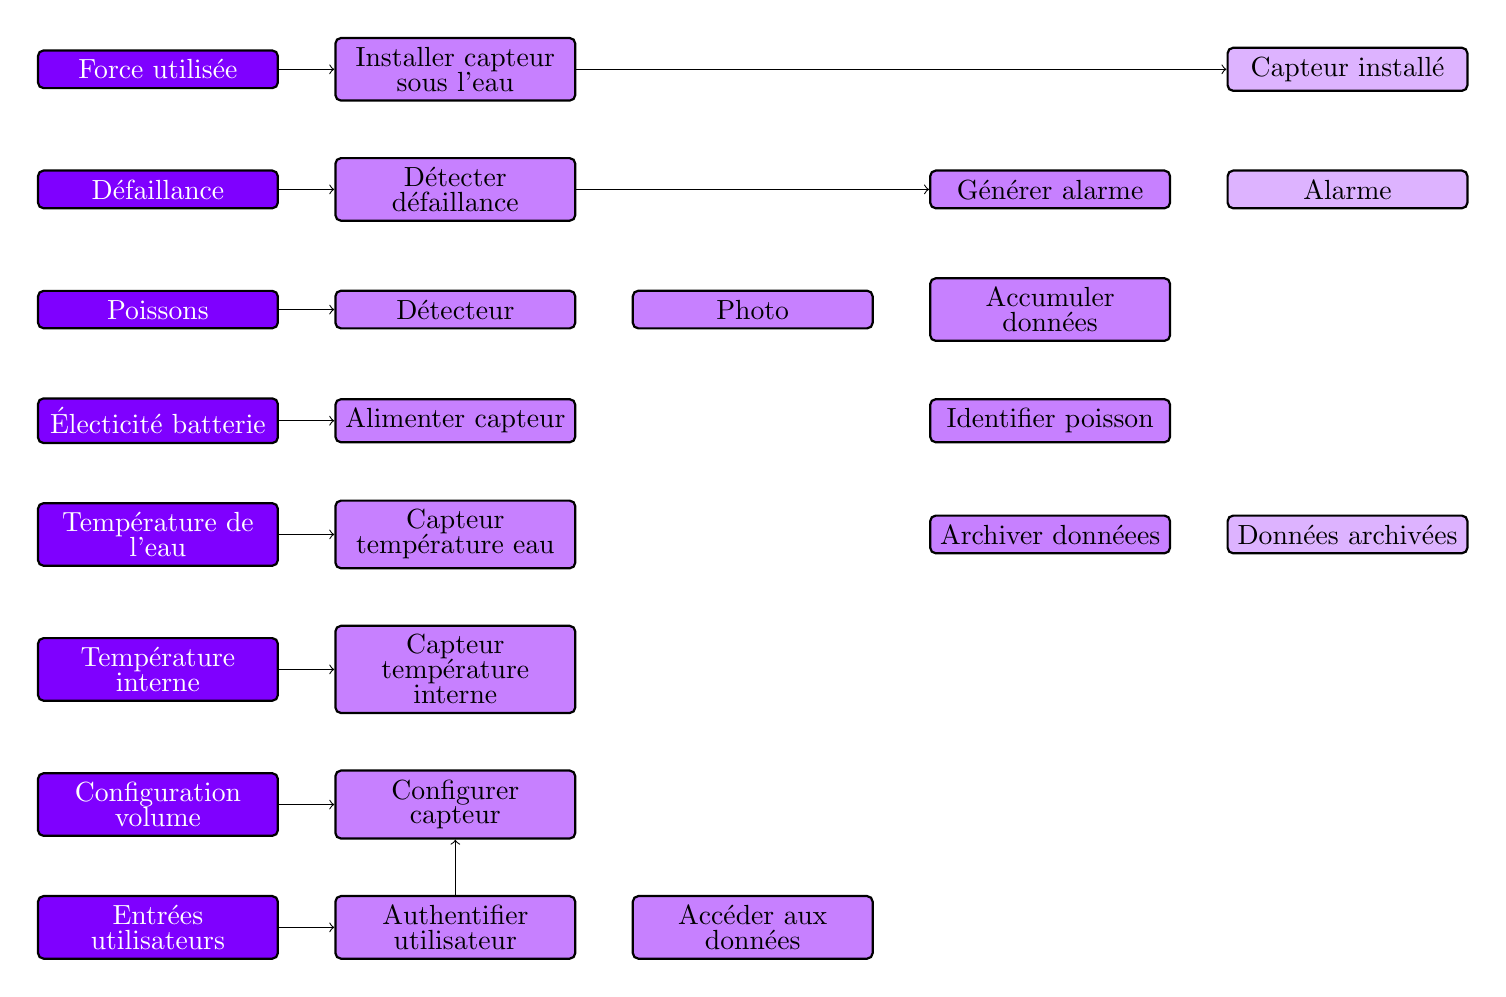
\begin{tikzpicture}[]
		\fontsize{10}{9} \selectfont
		% intrants
		\matrix[row sep=2em, column sep=2em] {
			% 1re ligne
			% TODO changer nom
			\node[intrant](forcutil){Force utilisée}; & \node[fonction](instcapt){Installer capteur sous l'eau}; & & & \node[extrant](captinst){Capteur installé}; \\
			% 2me ligne
			\node[intrant](defailla){Défaillance}; & \node[fonction](detcdefa){Détecter défaillance}; & & \node[fonction](genralrm){Générer alarme}; & \node[extrant](alarme){Alarme}; \\
			% 3me ligne
			\node[intrant](poissons){Poissons}; & \node[fonction](detecteu){Détecteur}; & \node[fonction](photo){Photo}; & \node[fonction](accudonn){Accumuler données}; & \\
			% 4me ligne
			\node[intrant](elecbatt){Électicité batterie}; & \node[fonction](alimcapt){Alimenter capteur}; & & \node[fonction](idenpois){Identifier poisson}; & \\
			% 5me ligne
			\node[intrant](tempreau){Température de l'eau}; & \node[fonction](captteau){Capteur température eau}; & & \node[fonction](archdonn){Archiver donnéees}; & \node[extrant](donnarch){Données archivées}; \\
			% 6me ligne
			\node[intrant](tempintr){Température interne}; & \node[fonction](capttcpt){Capteur température interne}; & & & \\
			% 7me ligne
			\node[intrant](confvolm){Configuration volume}; & \node[fonction](confcapt){Configurer capteur}; & & & \\
			% 8me ligne
			\node[intrant](entrutil){Entrées utilisateurs}; & \node[fonction](authutil){Authentifier utilisateur}; & \node[fonction](accedonn){Accéder aux données}; & & \\
		};
		
		% Liens
		\lienhorz{forcutil}{instcapt}
		\lienhorz{defailla}{detcdefa}
		\lienhorz{poissons}{detecteu}
		\lienhorz{elecbatt}{alimcapt}
		\lienhorz{tempreau}{captteau}
		\lienhorz{tempintr}{capttcpt}
		\lienhorz{confvolm}{confcapt}
		\lienhorz{entrutil}{authutil}
		
		\lienhorz{detcdefa}{genralrm}
		\lienhorz{instcapt}{captinst}
		
		\lienvtht{authutil}{confcapt}
	\end{tikzpicture}
	\caption{Diagramme fonctionnel}
	\label{f:caf_diag_fonc}
\end{figure}
\pagebreak
Le système à développer peut être décomposé en diverse fonctions. Chacune de ces fonction doit être explorée à travers par l'élaboration de différents concepts. Ces concepts permettrons d'obtenir un produit final optimal selon les exiges du MFA. D'abord, is faut isoler les composants du système du milieu aquatique pour assurer leur bon fonctionnement. Ensuite, les éléments du milieu (poissons, batterie, températures) sont mesurés afin d'être accumulés en mémoire. À partir de ces données, on peut identifier les poissons pris en photo pour ensuite archiver l'ensemble des données. Il est aussi important que les utilisateurs aient une méthode pour configurer le capteur et accéder aux données en archive. Tout ceci est décrit à la figure \ref{f:caf_diag_fonc}.

\section{Alimentation du système}

	Le système d’alimentation sera maintenu en surface par un système de flottaison. Afin de comprendre les choix de batterie nous étudions l’ampérage par heure qu’elle fournit en fonction des besoins énergétiques de notre système. Notre système doit au minimum être alimenté 14 jours soit 336 heures. En référence aux autres composants énergivores de notre système nous trouvons une consommation totale de 900 Ampère, auquel on alloue une marge d’erreur de 20\% pour tenir compte de la déperdition d’énergie. Soit 1080 Ampère au total. Par souci d’analyse nous calculons les besoins énergétiques ainsi que les caractéristiques globales de nos batteries pour 14, 16, 18 et 20 jours. Les concepts sont retenus en fonction du poids et volume totale ainsi que le prix. Les montages de batteries seront en parallèle afin d’avoir une sommation simplifié de l’ampérage total.\\

\begin{table}[htp]
\begin{tabular}{|c|c|c|c|c|}
\hline
                                                                                                & 14 jours & 16 jours & 18 jours & 20 jours \\ \hline
Heures                                                                                          & 336      & 384      & 432      & 480      \\ \hline
Ampères totale du système avec une marge de 20~\% (A) & 1080     & 1235     & 1390     & 1544     \\ \hline
\end{tabular}
\end{table}
	
	
	Consommation en ampère total du système pour 14 jours = [ 840A ( Ordinateur local) + 40.32A (Caméra) + 10.08A (Sonar) + 6.72A (Capteur de température) ] * 1.2 (marge d’erreur)

	    \subsection{Lithium Ion Battery - 18650 Cell}
\subsubsection{Description :} 
Une pile pesant 46 grammes pour un volume total de 21.53 cm3. Elle possède une capacité de 2,6 Ampères et à un prix de 7,93 dollars. Afin de répondre à nos besoins en énergie il en faut 415 unités.
\begin{table}[H]
\begin{tabular}{|c|c|c|c|c|c|}
\hline
Jours & Ampère & \begin{tabular}[c]{@{}c@{}}Nombre \\ batterie\end{tabular} & \begin{tabular}[c]{@{}c@{}}Poids \\ Total (kg)\end{tabular} & \begin{tabular}[c]{@{}c@{}}Volume \\ Total (cm3)\end{tabular} & \begin{tabular}[c]{@{}c@{}}Prix \\ Total (\$)\end{tabular} \\ \hline
14    & 1080   & 415                                                        & 19,09                                                       & 8934,95                                                       & 3290,95                                                    \\ \hline
16    & 1235   & 475                                                        & 21,85                                                       & 10226,75                                                      & 3766,75                                                    \\ \hline
18    & 1390   & 534                                                        & 24,56                                                       & 11497,02                                                      & 4234,62                                                    \\ \hline
20    & 1544   & 593                                                        & 27,28                                                       & 12767,29                                                      & 4702,49                                                    \\ \hline
\end{tabular}
\end{table}

\subsubsection{Décision :} Retenu, mais
\subsubsection{Justification :} Le poids est parfait pour une flottaison ainsi que son volume totale pour ne pas dégrader le paysage. Cependant le nombre important d’unité va demander un prix en main d’œuvre élevé pour établir le système.
\subsubsection{Référence : } 


\subsection{Lithium Ion Battery - 6Ah}
\subsubsection{Description :} 
Une batterie pesant 150 grammes pour un volume de 20.04 cm3. Elle possède une capacité de 6 Ampères et à un prix de 29,95 dollars. Afin de répondre à nos besoins en énergie il en faut 180 unités.

\begin{table}[!hbtp]
\begin{tabular}{|c|c|c|c|c|c|}
\hline
Jours & Ampère & Nombre batterie & Poids Total (kg) & Volume Total (cm3) & Prix Total (\$) \\ \hline
14    & 1080   & 180                                                        & 27                                                          & 3672                                                          & 5391            \\ \hline
16    & 1235   & 205                                                        & 30,75                                                       & 4182                                                          & 6139,75         \\ \hline
18    & 1390   & 231                                                        & 34,65                                                       & 4712,4                                                        & 6918,45         \\ \hline
20    & 1544   & 257                                                        & 38,55                                                       & 5242,8                                                        & 7697,15         \\ \hline
\end{tabular}
\end{table}

\subsubsection{Décision :} 
Retenu
\subsubsection{Justification :} 
Il y a un bon compromis entre poids, nombre d’unité et prix total.
\subsubsection{Référence : } 

\subsection{PANASONIC LC-R0612P}
\subsubsection{Description :} 
Une batterie pesant 2000 grammes pour un volume de 128.04 cm3. Elle possède une capacité de 12 Ampères et à un prix de 29,46 dollars. Afin de répondre à nos besoins en énergie il en faut 90 unités.\\
\begin{table}[!hbtp]
\begin{tabular}{|c|c|c|c|c|c|}
\hline
Jours & Ampère & Nombre batterie & Poids Total (kg) & Volume Total (cm3) &  Total (\$) \\ \hline
14    & 1080   & 90                                                         & 180                                                         & 11523,6                                                       & 2651,4                                                     \\ \hline
16    & 1235   & 102                                                        & 204                                                         & 13060,08                                                      & 3004,92                                                    \\ \hline
18    & 1390   & 115                                                        & 230                                                         & 14724,6                                                       & 3387,9                                                     \\ \hline
20    & 1544   & 128                                                        & 256                                                         & 16389,12                                                      & 3770,88                                                    \\ \hline
\end{tabular}
\end{table}

\subsubsection{Décision :} 
Non retenu
\subsubsection{Justification :} 
Le poids total est beaucoup trop élevé pour un système de flottaison
\subsubsection{Référence : } 

\subsection{Batterie rechargeable Lithium-Ion RS PRO}
\subsubsection{Description :} 
Une batterie pesant 186 grammes pour un volume de 94,32 cm3. Elle possède une capacité de 10,4 Ampères et à un prix de 58,63 dollars. Afin de répondre à nos besoins en énergie il en faut 103 unités.
\begin{table}[!hbtp]
\begin{tabular}{|c|c|c|c|c|c|}
\hline
Jours & Ampère & \begin{tabular}[c]{@{}c@{}}Nombre \\ batterie\end{tabular} & \begin{tabular}[c]{@{}c@{}}Poids \\ Total (kg)\end{tabular} & \begin{tabular}[c]{@{}c@{}}Volume \\ Total (cm3)\end{tabular} & \begin{tabular}[c]{@{}c@{}}Prix \\ Total (\$)\end{tabular} \\ \hline
14    & 1080   & 103                                                        & 18,85                                                       & 9714,96                                                       & 6038,89                                                    \\ \hline
16    & 1235   & 118                                                        & 21,59                                                       & 11129,76                                                      & 6918,34                                                    \\ \hline
18    & 1390   & 133                                                        & 24,34                                                       & 12544,56                                                      & 7797,79                                                    \\ \hline
20    & 1544   & 148                                                        & 27,08                                                       & 13959,36                                                      & 8677,24                                                    \\ \hline
\end{tabular}
\end{table}

\subsubsection{Décision :} 
Retenu, mais
\subsubsection{Justification :} 
Le faible poids est intéressant pour le système de flottaison.\\ Cependant le prix reste un peu élevé sans compter la main d’œuvre pour concevoir le système.
\subsubsection{Référence : } 

% !TeX encoding = UTF-8
% !TeX spellcheck = fr_FR


\section{Archiver les données}
\label{s:faisab_archiver}
Le MFA exige que l’ensemble des données soient conservées pour un minimum de deux ans. Les données sont constituées des éléments suivants: images originales, vignettes, identification, date et heure, température du système, température de l’eau et alarmes. La capacité en mémoire et la fiabilité doivent donc être suffisants pour garantir l’intégrité des données sur 2 ans.

Aspects physiques:
-Le concept doit avoir assez de mémoire pour conserver 2 années d'information: 1 To.
-Le concept doit être assez fiable pour garantir l’intégrité des données sur 2 ans.
Aspects économiques:
-Le concept doit minimiser le coût 
Aspects temporels:
-Le concept doit pouvoir être construit et déployé dans les délais du projets.
Aspects sociaux-environnementaux:
-Non-applicable


% !TeX encoding = UTF-8
% !TeX spellcheck = fr_FR


\subsection{Serveur PowerEdge T30}
\label{s:archiver_conc1}

\textbf{Description}:La compagnie Dell offre un serveur prêt à accepter jusqu’à 4 disques durs pour 604,80\$. Ce serveur sera installé au MFA. Le montant inclut une garantie de 2 ans sur le matériel avec livraison le jour suivant. En ajoutant 2 disques durs Western Digital Red de 1 To pour 149,98\$ branchés en RAID1, on a 1 To de mémoire redondante. Ces disques ont un temps moyen entre pannes de 1000000 h, c-à-d 114 années.  Le coût total du matériel se limite à 754,68\$. 
\textbf{Décision}: Retenu mais 
\textbf{Justification}: Ce matériel permet d’entreposer une quantité suffisante de données. Le matériel du serveur est garanti sur 2 ans. Les disques durs de 1 To ont une cote de fiabilité dépassant largement 2 ans, en plus d’être installés de manière redondante. Les données n’ont toutefois aucune redondance géographique, ce qui augmente le risque de perte de données. Toutes les composantes sont disponibles immédiatement. Le coût total est acceptable dans le contexte du projet.
\textbf{Références}:
\cite{dellT30, amazonWDred, wdRedSpec, wiki_raid1}



% !TeX encoding = UTF-8
% !TeX spellcheck = fr_FR


\subsection{Serveur PowerEdge T30}
\label{s:archiver_conc1}

\textbf{Description}:La compagnie Dell offre un serveur prêt à accepter jusqu’à 4 disques durs pour 604,80\$. Ce serveur sera installé au MFA. Le montant inclut une garantie de 2 ans sur le matériel avec livraison le jour suivant. En ajoutant 2 disques durs Western Digital Red de 1 To pour 149,98\$ branchés en RAID1, on a 1 To de mémoire redondante. Ces disques ont un temps moyen entre pannes de 1000000 h, c-à-d 114 années.  Le coût total du matériel se limite à 754,68\$. 
\textbf{Décision}: Retenu mais 
\textbf{Justification}: Ce matériel permet d’entreposer une quantité suffisante de données. Le matériel du serveur est garanti sur 2 ans. Les disques durs de 1 To ont une cote de fiabilité dépassant largement 2 ans, en plus d’être installés de manière redondante. Les données n’ont toutefois aucune redondance géographique, ce qui augmente le risque de perte de données. Toutes les composantes sont disponibles immédiatement. Le coût total est acceptable dans le contexte du projet.
\textbf{Références}:
\cite{dellT30, amazonWDred, wdRedSpec, wiki_raid1}



% !TeX encoding = UTF-8
% !TeX spellcheck = fr_FR


\subsection{Serveur PowerEdge T30}
\label{s:archiver_conc1}

\textbf{Description}:La compagnie Dell offre un serveur prêt à accepter jusqu’à 4 disques durs pour 604,80\$. Ce serveur sera installé au MFA. Le montant inclut une garantie de 2 ans sur le matériel avec livraison le jour suivant. En ajoutant 2 disques durs Western Digital Red de 1 To pour 149,98\$ branchés en RAID1, on a 1 To de mémoire redondante. Ces disques ont un temps moyen entre pannes de 1000000 h, c-à-d 114 années.  Le coût total du matériel se limite à 754,68\$. 
\textbf{Décision}: Retenu mais 
\textbf{Justification}: Ce matériel permet d’entreposer une quantité suffisante de données. Le matériel du serveur est garanti sur 2 ans. Les disques durs de 1 To ont une cote de fiabilité dépassant largement 2 ans, en plus d’être installés de manière redondante. Les données n’ont toutefois aucune redondance géographique, ce qui augmente le risque de perte de données. Toutes les composantes sont disponibles immédiatement. Le coût total est acceptable dans le contexte du projet.
\textbf{Références}:
\cite{dellT30, amazonWDred, wdRedSpec, wiki_raid1}



% !TeX encoding = UTF-8
% !TeX spellcheck = fr_FR


\subsection{Serveur PowerEdge T30}
\label{s:archiver_conc1}

\textbf{Description}:La compagnie Dell offre un serveur prêt à accepter jusqu’à 4 disques durs pour 604,80\$. Ce serveur sera installé au MFA. Le montant inclut une garantie de 2 ans sur le matériel avec livraison le jour suivant. En ajoutant 2 disques durs Western Digital Red de 1 To pour 149,98\$ branchés en RAID1, on a 1 To de mémoire redondante. Ces disques ont un temps moyen entre pannes de 1000000 h, c-à-d 114 années.  Le coût total du matériel se limite à 754,68\$. 
\textbf{Décision}: Retenu mais 
\textbf{Justification}: Ce matériel permet d’entreposer une quantité suffisante de données. Le matériel du serveur est garanti sur 2 ans. Les disques durs de 1 To ont une cote de fiabilité dépassant largement 2 ans, en plus d’être installés de manière redondante. Les données n’ont toutefois aucune redondance géographique, ce qui augmente le risque de perte de données. Toutes les composantes sont disponibles immédiatement. Le coût total est acceptable dans le contexte du projet.
\textbf{Références}:
\cite{dellT30, amazonWDred, wdRedSpec, wiki_raid1}



% !TeX encoding = UTF-8
% !TeX spellcheck = fr_FR


\begin{table}[!htbp]
	\begin{tabular}{|l|c|c|c|c|c|}
		\hline
		\multicolumn{1}{|c|}{\multirow{2}{*}{\textbf{Concepts}}} & \multicolumn{4}{c|}{\textbf{Aspects de l'analyse}} & \multirow{2}{*}{\textbf{Décision}} \\ \cline{2-5}
		\multicolumn{1}{|c|}{}                                   & Physiques & Économiques & Temporels & Socio-envir. &                                    \\ \hline
		Serveur PowerEdge T30                                                 & OUI MAIS       & OUI         & OUI       & OUI          & RETENU MAIS                             \\ \hline
		Service nuagique Amazon S3                                                 & OUI       & OUI         & OUI       & OUI          & RETENU                             \\ \hline
		Service nuagique Microsoft Azure                                                 & OUI       & OUI         & OUI       & OUI          & RETENU                             \\ \hline
		Serveur dédié chez OVH                                                & OUI MAIS      & OUI MAIS        & OUI       & OUI          & RETENU MAIS        \\ \hline
	\end{tabular}
	\caption{Décisions pour fonction "archiver les données"}
	\label{tab:fct_archiver}
\end{table}

% !TeX encoding = UTF-8
% !TeX spellcheck = fr_FR


\section{Identifier les espèces de poissons}
\label{s:faisab_identifier}
Le MFA exige pouvoir identifier 5 espèces de poissons identifiables par site étudié. L’identification doit être faite de manière autonome partir d’une vignette 100 par 100 pixels. Les concepts retenus doivent non seulement identifier les espèces mais offrir niveau de fiabilité acceptable. L’apprentissage automatique (de l’anglais “machine learning”) semble être la technologie à favoriser dans notre cas. Le choix de plateforme pour l’apprentissage automatique devrait minimiser le coût et le temps de développement.

Puisqu’il n’existe pas de banque d’image permettant d’entraîner la machine pour cette tâche, une telle collection devra être créée pour le projet. Environ 200 images identifiées par espèce devraient suffir pour entraîner l’algorithme.\cite{deeplearn_2015, fishID_2016} Faire classifier 200 images par un biologiste devrait prendre au plus 1 journée, pour un total de 240\$ \cite{sal_biologiste} par espèce. Les images à identifier manuellement proviendront des premières images générées par le projet. Accumuler 200 images d’une nouvelle espèce pourrait prendre jusqu’à 1 mois, mais s’effectue en parallèlement pour toutes les espèces d’un milieu particulier.

Aspects physiques:
-L’identification doit pouvoir être fiable (REF fiabilité?)
Doit pouvoir identifier au minimum 5 espèces de poisson.
Aspects économiques:
-Limiter le coût de développement.
-Limiter le coût d’achat de matériel, si applicable. (??)
Aspects temporels:
-Le concept doit pouvoir être développé dans les délais du projet.
Aspects sociaux-environnementaux:
-Non-applicable.


% !TeX encoding = UTF-8
% !TeX spellcheck = fr_FR


\subsection{TensorFlow sur Google Cloud}
\label{s:identifier_conc1}

\textbf{Description}:TensorFlow est la plateforme “open source” d'apprentissage automatique de Google. L’utilisation de TensorFlow est gratuite en respectant la licence [ref:liscapache2]. Avec une banque d’image pré-identifiées, 3 semaines de travail sont estimée pour développer l'algorithme d’apprentissage et l’entraîner. Ceci coûtera environ 4615\$, selon le salaire moyen d’un ingénieur logiciel[ref:salingLog]. Dans ces conditions la fiabilité de l’identification devrait approcher 95\%[ref:fishID_2016]. Googl Cloud est un service nuagique qui permet l’apprentissage automatique. Faire fonctionner cet algorithme sur Google Cloud pendant 2 ans devrait coûter aux environs de 2200\$. Développer un banque d’images pour 5 espèces monte à 1200\$ et 1 semaine de travail. Incluant la banque d’image, ce concept nécessitera donc un total de 4 semaines de travail, 2200\$ en matériel et 5815\$.
\textbf{Décision}: Retenu
\textbf{Justification}: Les coût de développement et de matériel sont en raisonnables. Les ressources choisies sont appropriées pour obtenir une identification fiable d’un nombre approprié d’espèces. Un mois de développement est acceptable dans le cadre du projet.
\textbf{Références}: googCloud, tensorFlow
% !TeX encoding = UTF-8
% !TeX spellcheck = fr_FR


\subsection{TensorFlow sur Google Cloud}
\label{s:identifier_conc1}

\textbf{Description}:TensorFlow est la plateforme “open source” d'apprentissage automatique de Google. L’utilisation de TensorFlow est gratuite en respectant la licence [ref:liscapache2]. Avec une banque d’image pré-identifiées, 3 semaines de travail sont estimée pour développer l'algorithme d’apprentissage et l’entraîner. Ceci coûtera environ 4615\$, selon le salaire moyen d’un ingénieur logiciel[ref:salingLog]. Dans ces conditions la fiabilité de l’identification devrait approcher 95\%[ref:fishID_2016]. Googl Cloud est un service nuagique qui permet l’apprentissage automatique. Faire fonctionner cet algorithme sur Google Cloud pendant 2 ans devrait coûter aux environs de 2200\$. Développer un banque d’images pour 5 espèces monte à 1200\$ et 1 semaine de travail. Incluant la banque d’image, ce concept nécessitera donc un total de 4 semaines de travail, 2200\$ en matériel et 5815\$.
\textbf{Décision}: Retenu
\textbf{Justification}: Les coût de développement et de matériel sont en raisonnables. Les ressources choisies sont appropriées pour obtenir une identification fiable d’un nombre approprié d’espèces. Un mois de développement est acceptable dans le cadre du projet.
\textbf{Références}: googCloud, tensorFlow
% !TeX encoding = UTF-8
% !TeX spellcheck = fr_FR


\subsection{TensorFlow sur Google Cloud}
\label{s:identifier_conc1}

\textbf{Description}:TensorFlow est la plateforme “open source” d'apprentissage automatique de Google. L’utilisation de TensorFlow est gratuite en respectant la licence [ref:liscapache2]. Avec une banque d’image pré-identifiées, 3 semaines de travail sont estimée pour développer l'algorithme d’apprentissage et l’entraîner. Ceci coûtera environ 4615\$, selon le salaire moyen d’un ingénieur logiciel[ref:salingLog]. Dans ces conditions la fiabilité de l’identification devrait approcher 95\%[ref:fishID_2016]. Googl Cloud est un service nuagique qui permet l’apprentissage automatique. Faire fonctionner cet algorithme sur Google Cloud pendant 2 ans devrait coûter aux environs de 2200\$. Développer un banque d’images pour 5 espèces monte à 1200\$ et 1 semaine de travail. Incluant la banque d’image, ce concept nécessitera donc un total de 4 semaines de travail, 2200\$ en matériel et 5815\$.
\textbf{Décision}: Retenu
\textbf{Justification}: Les coût de développement et de matériel sont en raisonnables. Les ressources choisies sont appropriées pour obtenir une identification fiable d’un nombre approprié d’espèces. Un mois de développement est acceptable dans le cadre du projet.
\textbf{Références}: googCloud, tensorFlow
% !TeX encoding = UTF-8
% !TeX spellcheck = fr_FR


\subsection{TensorFlow sur Google Cloud}
\label{s:identifier_conc1}

\textbf{Description}:TensorFlow est la plateforme “open source” d'apprentissage automatique de Google. L’utilisation de TensorFlow est gratuite en respectant la licence [ref:liscapache2]. Avec une banque d’image pré-identifiées, 3 semaines de travail sont estimée pour développer l'algorithme d’apprentissage et l’entraîner. Ceci coûtera environ 4615\$, selon le salaire moyen d’un ingénieur logiciel[ref:salingLog]. Dans ces conditions la fiabilité de l’identification devrait approcher 95\%[ref:fishID_2016]. Googl Cloud est un service nuagique qui permet l’apprentissage automatique. Faire fonctionner cet algorithme sur Google Cloud pendant 2 ans devrait coûter aux environs de 2200\$. Développer un banque d’images pour 5 espèces monte à 1200\$ et 1 semaine de travail. Incluant la banque d’image, ce concept nécessitera donc un total de 4 semaines de travail, 2200\$ en matériel et 5815\$.
\textbf{Décision}: Retenu
\textbf{Justification}: Les coût de développement et de matériel sont en raisonnables. Les ressources choisies sont appropriées pour obtenir une identification fiable d’un nombre approprié d’espèces. Un mois de développement est acceptable dans le cadre du projet.
\textbf{Références}: googCloud, tensorFlow
% !TeX encoding = UTF-8
% !TeX spellcheck = fr_FR


\subsection{Tableau identifier}
\label{s:archiver_tableau}



% !TeX encoding = UTF-8
% !TeX spellcheck = fr_FR


\section{Accumuler les données}
\label{s:faisab_accumuler}

Un dispositif local est nécessaire afin de coordonner tous les composantes. Notre système doit avoir un ordinateur localement afin de permettre de gérer toutes l’information qui proviennent des divers composantes soit: la caméra, les thermomètres, le sonar, le niveau d’alimentation de la batterie, les entrées de l’utilisateur à distance et la détection d’un malfonctionnement au niveau de ces composantes. D’ailleurs, l’ordinateur possèdera un espace de stockage de 64 Go localement, soit une carte Micro SD sandisk 64Gb à 15.71\$ qui sera livrée en deux jours, afin de pouvoir conserver les logiciels nécessaires au fonctionnement du système et de conserver les photos temporairement afin de les envoyer vers le API qui traitera les photos et détectera les poissons. De plus, l’ordinateur doit être en mesure d’envoyer les photos qu’il stocke et reçoit de la caméra pour les transférer au logiciel de traitement et envoyer les alarmes à l’utilisateur du système. C’est pourquoi une antenne wifi puissante lui sera assignée afin de pouvoir communiquer à l’opérateur situé à 1km de distance (l’antenne communiquera avec internet, donc le API, avec le poste de l’opérateur). Cette antenne sera la Antenna World G2424 qui s’élève à 149\$ et qui transmet le réseau wifi à une distance de 10 km. Les critères de faisabilités des concepts pour cette section sont évalués selon les aspects suivants:

Aspects physiques:
\begin{itemize}
	\item Le système doit être assez petit pour être dans le contenant d’étanchéité du système
	\item Le système doit contenir assez d’entrées pour tous les périphériques du système
\end{itemize}

Aspects économiques:
\begin{itemize}
	\item Minimiser les coûts de l’ordinateur
\end{itemize}

Aspects temporels:
\begin{itemize}
	\item L’ordinateur doit pouvoir être implanté dans les délais du projets.
\end{itemize}

Aspects sociaux-environnementaux:
\begin{itemize}
	\item L’ordinateur doit avoir la consommation électrique la plus faible possible
\end{itemize}

\subsection{Raspberry pi 3 B+}

\textbf{Description}: Le Raspberry Pi 3 B+ est un microcontrôleur avec un processeur Broadcom BCM2837B0, Cortex-A53 64 bit qui génère une fréquence 1.4 GHz. Le processeur utilise une architecture ARMv8 et à 1Gb de SDRAM. Il possède aussi une carte LAN, Bluetooth 4.2 et BLE à deux fréquences soit 2.4 GHz et 5GHz. De plus, il possède quatres ports USB 2.0, un port HDMI, un port CSI pour connecter une caméra,  et un header GPIO de 40 pins. Il est possible d’installer n’importe quel système d’exploitation sur ce microcontrôleur et il vient préinstallé avec une distribution de linux spécifique aux Raspberry Pi soit une version Debian de Linux. Le Pi possède aussi un GPU pour un traitement de base des images et sa température d’opération est entre 0 et 50 degré Celsius. Il est à noter aussi que la consommation en électricité de cette carte est très faible malgré ses nombreuses composantes. Le coût de cette composante est 47.95\$ ce qui est un microcontrôleur entrée de gamme.

\textbf{Décision}: Retenue

\textbf{Justification}: Ce concept est retenu, car il comble tous les critères établis précédemment. De plus, la gamme de produits Raspberry Pi est reconnue dans l’industrie de l’informatique comme des microcontrôleurs, fiables, petits et performants.


\subsection {ASUS Tinker Board}

\textbf{Description}: Le ASUS Tinker Board est un microcontrôleur très performant avec un microprocesseur Rockchip RK3288 à quatres coeurs avec une architecture ARM et 1.8GHz de fréquence. Il possède aussi 2GB de DDR3 Ram et une carte wifi et bluetooth performante qui peut s’améliorer avec une antenne externe IPEX à 6.53\$. Le Tinker Board offre aussi un Mali-T764 comme GPU qui offre 16 coeurs et 600MHz comme vitesse d’horloge. Comme connections, ASUS offre 4 ports USB 2.0, une connection pour un cable HDMI, une connection auxiliaire 3.5mm et une connection MIPI DSI pour les connections analogues. Le microcontrôleur utilise une carte microSD pour stocker les données en mémoire et utilise TinkerOS comme système d’exploitation, une distribution Debian de Linux qui est préprogrammée avec le système. Le coût de l’ordinateur est 88.26\$ ce qui le place dans le milieu de la gamme des microcontrôleurs.

\textbf{Décision}: Retenue

\textbf{Justification}: Ce concept est retenu, car il respecte tous les critères établis précedemment. Le Tinker Board ce distingue des autres microcontrôleur par sa performance il est le plus performant de sa gamme avec une composition axée sur les opérations plus lourdes au niveau du processeur.

\subsection {Odroid-C2}

\textbf{Description}:
Le Odroid-C2 est un microcontrôleur qui possède un processeur Amlogic S905 à quatre coeurs qui offre 1.5Ghz de fréquence. Il possède aussi un Mali-450 MP2 comme GPU et 2Go de RAM inclus et l’option de mettre 8Go de RAM. Le Odroid offre 4 ports USB, une connection ethernet, un port HDMI, 40 entrées analogues et une sortie 4K 60Hz vidéo. De plus, ce microcontrôleur a une très faible consommation en énergie. Il est possible d’installer Ubuntu 16.04 ou Android 6.0 Marshmallow comme système d’exploitation. Le coût de l’ordinateur est de 46\$ ce qui le place dans la même gamme que le Raspberry Pi 3B+.

\textbf{Décision}: Retenue

\textbf{Justification}: Ce concept est retenu, car il respecte tous les critères établis précedemment et il est une excellente alternative au Raspberry Pi 3B+.

\subsection {UDOO x86 ADVANCED PLUS}

\textbf{Description}: Le UDOO x86 ADVANCED PLUS est un des microcontrôleurs les plus puissants sur le marché. Il possède un microprocesseur Intel Celeron N3160 avec quatre coeurs et 2.24 GHz de fréquence et 4GB de DDR3L Dual Channel RAM. Il possède une carte graphique comparable à celles dans les ordinateurs portables modernes soit une Intel HD Graphics 400 qui peut monter jusqu’à 640 MHz de vitesse d’horloge. Le système possède une connection HDMI et deux connections miniDP++. De plus, le UDOO vient avec 32Go de mémoire inclus dans la carte mère, une fente M.2 Key B SSD et une fente pour insérer une carte microSD supplémentaire. Le système ne vient pas avec une carte Wifi intégrée comme les autres, mais elle a la possibilité d’être rajoutée et elle vient avec une connection ethernet. D’ailleurs, 3 ports USB 3.0 sont sur la carte-mère ainsi que deux connections UART et une connection auxiliaire pour le son. Il possède 20 entrées analogues GPIO et il peut utiliser Windows, n’importe quelle distribution de Linux et Android comme système d’exploitation. Par ailleurs, le UDOO possède deux parties soit une partie qui est comme un ordinateur et une partie qui est comme un microcontrôleur Arduino avec une connection directe entre le logiciel et les sorties analogues et il possède aussi des senseurs pour détecter l’accélération et un gyroscope. Le coût du UDOO x86 ADVANCED PLUS est de 174\$ c’est donc un microcontrôleur haut de gamme.

\textbf{Décision}: Rejetée

\textbf{Justification}: Même si ce microcontrôleur possède beaucoup d’options et de fonctionnalités et est très performant, la plupart des ces fonctionnalités ne seront pas utilisées pour le projet Fish and Chips étant donné de la nature de celui-ci. Ainsi, il serait plus justifiable d’aller avec un autre microcontrôleur moins cher avec moins de fonctionnalités mais qui est tout de même capable d’accomplir le travail nécessaire.

\begin{table}[!htbp]
	\begin{tabular}{|l|c|c|c|c|c|}
	\hline
	\multicolumn{1}{|c|}{\multirow{2}{*}{\textbf{Concepts}}} & \multicolumn{4}{c|}{\textbf{Aspects de l'analyse}} & \multirow{2}{*}{\textbf{Décision}} \\ \cline{2-5}
	\multicolumn{1}{|c|}{}                                   & Physiques & Économiques & Temporels & Socio-envir. &                                    \\ \hline
	Raspberry pi 3 B+                                                 & OUI       & OUI         & OUI       & OUI          & RETENU                             \\ \hline
	ASUS Tinker Board                                               & OUI       & OUI         & OUI       & OUI          & RETENU                             \\ \hline
	Odroid-C2                                                 & OUI       & OUI         & OUI       & OUI          & RETENU                             \\ \hline
	UDOO X86 ADVANCED PLUS                                               & OUI       & NON         & OUI       & NON         & REJETÉ	        \\ \hline
	\end{tabular}
	\caption{Décisions pour fonction "accumuler les données"}
	\label{tab:fct_acceder}
\end{table}

% !TeX encoding = UTF-8
% !TeX spellcheck = fr_FR


\section{Accéder aux données}
\label{s:faisab_acceder}
Pour assurer une connexion en en tout temps avec le système, une interface d’utilisateur intuitive et simple pour quelqu’un qui n’a pas de connaissances avancées en informatique pour procurer un accès à distance sécurisé sur le dispositif pour permettre au technicien d’effectuer des configurations. Le système Fish and Chips doit donc être en mesure de publier les informations en temps réel pour que le technicien puisse voir l’état du système et il doit voir une alarme lors d’un malfonctionnement du système. L’accès au système doit être rapide et doit se faire dans un rayon de 1 km du système. Les critères de faisabilités pour cette section sont évalués selon les aspects suivants :

Aspects physiques:
\begin{itemize}
	\item L’interface du système doit être simple d’utilisation pour quelqu’un qui n’est pas spécialisé en informatique
	\item L’interface doit être accessible partout et en tout temps
\end{itemize}

Aspects économiques:
\begin{itemize}
	\item Minimiser le coût d’implantation du concept
\end{itemize}

Aspects temporels:
\begin{itemize}
	\item L’interface doit pouvoir être implanté dans les délais du projet
\end{itemize}

Aspects sociaux-environnementaux:
\begin{itemize}
	\item L’accès à l’interface doit être sécurisé
\end{itemize}

\subsection{Connection SSH avec le dispositif Fish and Chips et interface graphique sur localhost développée par un tiers}

\textbf{Description}:
Une connection SSH est une alternative qui est utilisée très fréquemment pour se connecter à un ordinateur ou un robot à distance, elle procure un accès sécurisé qui permet n’importe qui avec le mot de passe de se connecter au dispositif. Une fois que la connection est établie entre l’ordinateur de l’opérateur et du système une interface graphique s’affiche dans n’importe quel fureteur web à l’adresse localhost:4000 et de cet interface, l’opérateur peut voir: l’état du système, si des alarmes ont été soulevés et si la détection de poissons s’effectue avec succès. D’ailleurs, pour les alarmes, un système qui relie le numéro de cellulaire de l’opérateur et le système en lui envoyant un message “texto” est de mise pour signaler une alarme. Cette fonctionnalité permettrait de le contacter n’importe où pour régler le malfonctionnement du système. Le coût de développement pour le système est faible étant donné qu’aucun serveur doit être utilisé à l’externe, que l’interface graphique n’est pas complexe et que la connectivité SSH est déja établie sur presque tous les systèmes d’exploitation. De plus, le temps de développement est aussi petit, soit 15 semaines, dû à la petite quantité de programmes qui sont développés. Pour un interface web tel que spécifié ci-haut le coût s’élèverait à 20000\$.

\textbf{Décision}: Retenue

\textbf{Justification}: La connection SSH est une connection simple, sécurisée et qui permet d’éviter de mettre du temps de développement sur la connection, mais plutôt d’investir le temps dans un interface graphique de qualité.

\subsection {Connection en passant par une application web développée par un tiers}

\textbf{Description}: Une autre solution consiste à employer des programmeurs qui développeront une application web listée qui sera accessible par une authentification sur la page d'accueil. La page web sera disponible sur un ordinateur normal et sur un cellulaire en utilisant HTML5 et elle sera conforme avec toutes les plateformes sans avoir besoin d’investir du temps dans une compatibilité globale. De plus, la connection se fait directement avec le système Fish and Chips après l’authentification de l’opérateur. Pour la sécurité, l’utilisateur du site sera demandé de s’authentifier sur la page d’acceuil pour avoir accès au Fish and Chips et la seule manière d’y avoir accès est d’avoir un mot de passe qui sera transmis à l’opérateur seulement. La base de donnée utilisé est MySQL vu qu’elle est simple, mais elle est potentiellement dangereuse. C’est pourquoi pour la sécurité de la base de données, une attention particulière est de mise et le développement se conforme au protocole OWASP et l’accès au site web est encrypté afin d'empêcher l’interception du trafic. La durée de conception est de 25 semaines. Le coût est aux alentours de 30000\$ et c’est un prix qui inclut tous les éléments nécessaires au fonctionnement de l’interface.

\textbf{Décision} : Retenue

\textbf{Justification}: Cette option est la plus simple pour l’opérateur, car elle nécessite aucune connaissance en informatique, car celui-ci aura seulement besoin de se connecter sur le site web et s’authentifier pour avoir accès au système.

\subsection {Programme local et application mobile développée par un tiers}

\textbf{Description}:
Une autre solution consiste à employer des développeurs pour créer deux applications locales soit une sur un ordinateur et une sur un téléphone cellulaire. Cette solution est une variante de la connection SSH dénotée plus haut, mais est une application à part entière plutôt que de faire appel à un fureteur web marchant sur localhost. L’avantage de cette solution est que comme l’application est téléchargée localement et effectue un contact direct en SSH avec le système le coût de développement en sécurité est très faible. De plus, l’utilisation est extrêmement simple l'exécution du programme se connecte directement avec le système pour ensuite afficher un interface graphique en local. Comme cette solution n’est pas portable il faut compiler un exécutable fait pour le système d’exploitation qu’ utilisera l’opérateur. Par contre, il faut créer une version pour une application mobile afin d’assurer le transfert des alarmes avec l’opérateur ce qui rajoute des coûts et du temps de développement. Ainsi, le temps de développement serait d'environ 30 semaines et les coûts d’environ 35000\$ ce qui est aux limites de notre budget.

\textbf{Décision}: Retenue

\textbf{Justification}: Cette alternative peut être efficace si nous tentons de minimiser les connections avec internet dans notre projet. Même si ce concept n’est pas le plus récent en manière de technologie, elle respecte quand même tous les critères et c’est pourquoi elle est retenue.

\subsection {SSH avec une application dans la ligne de commande développée par un tiers}

\textbf{Description}:
La dernière solution consiste à construire une application qui a beaucoup de fonctionnalités et qui fonctionnera directement dans la ligne de commande. L’avantage de cette solution est que les coûts de développement sont très faible dû à l’abstention d’interface graphique en faisant appel à diverses commandes qui sont exécutés pour avoir un accès direct aux données et à l’état du système en l’imprimant dans le terminal. Par contre, l’inconvénient de cette solution est que pour utiliser cet interface efficacement il faut certaine connaissances en informatique que l’opérateur n’aura pas nécessairement. Le coût de développement de cette application serait faible soit environ 20000\$ dû à l’économie de temps qui surviendra d’éviter le développement d’un interface graphique et le temps de développement est de 20 semaines.

\textbf{Décision}: Rejetée

\textbf{Justification}: Cette interface exige des bonnes connaissances en informatique et tel que cité dans les aspects physiques, il est nécessaire de choisir un interface qui ne requiert pas des connaissances poussées en informatique.

\begin{table}[!htbp]
	\begin{tabular}{|l|c|c|c|c|c|}
		\hline
		\multicolumn{1}{|c|}{\multirow{2}{*}{\textbf{Concepts}}} & \multicolumn{4}{c|}{\textbf{Aspects de l'analyse}} & \multirow{2}{*}{\textbf{Décision}} \\ \cline{2-5}
		\multicolumn{1}{|c|}{}                                   & Physiques & Économiques & Temporels & Socio-envir. &                                    \\ \hline
		Connexion SSH                                                  & OUI       & OUI         & OUI       & OUI          & RETENU                             \\ \hline
		Application web                                                 & OUI       & OUI         & OUI       & OUI          & RETENU                             \\ \hline
		Programme local et application mobile                                                & OUI       & OUI         & OUI       & OUI          & RETENU                             \\ \hline
		Ligne de commande                                                 & NON       & OUI         & OUI       & OUI          & REJETÉE	        \\ \hline
	\end{tabular}
	\caption{Décisions pour fonction "accéder aux données"}
	\label{tab:fct_acceder}
\end{table}

\section{Prendre une photo}
	
	Pour la caméra, il est important, qu’elle ne consomme pas trop d’énergie, qu’elle soit plutôt compacte, car nous disposons d’un espace limité. Il faut aussi que la caméra puisse prendre des photos en au moins 16 pixels et 8 bits afin de pouvoir identifier l’espèce du poisson. Il est intéressant d’aussi tenir en compte des spécificités uniques aux différentes caméra, par exemple si celle-ci est déjà étanche.
	
	Aspects physiques:
	\begin{itemize}
		
		\item Il faut que la caméra prenne des photos en au moins 8 bits et 16 pixels.
		
	\end{itemize}
	
	Aspects économiques :
	
	\begin{itemize}
		
		\item Nous devons nous assurer que le prix est minimal.
		
	\end{itemize}
	
	Aspects temporels:
	
	\begin{itemize}
		\item La caméra doit avoir une autonomie suffisamment basse pour être considéré comme une option viable.		
		\item La livraison doit être faite dans un délais raisonnable.
	\end{itemize}

	Aspects socio-économiques:
	\begin{itemize}
	\item Non-applicable.
	\end{itemize}
	
	\subsection{Mini caméra Full HD 1080P DV sok3254}
	

	\textbf{Description}: Cette caméra à une volume de 1 pouce cube, ce qui n’est pas trop gros et permet de réduire la taille du modèle. La caméra possède une résolution de 1920 X 1080p, alors la qualité de l’image n’est pas un problème. La caméra permet une prise de photo à 150 degrés afin de maximiser l’information prise en une photo. Cette caméra a aussi un système de 6 LED intégré afin de prendre des photos la nuit ou en l'absence de lumières, ce qui est bénéfique pour faciliter le fonctionnement du système complet. Ensuite la caméra possède une mémoire de 32 gigaoctets, ce qui amplement suffisant pour la tâche demandée. Finalement, la caméra possède une autonomie de 7 jours, avec une batterie au lithium-ion de 200 milliampère par heure (mAh), ce qui est suffisant sachant que la caméra peut prendre des photos lors de la charge et que notre système comportera une batterie qui pourra recharger la caméra pour les 7 jours manquant. Le prix de cette caméra est de 14\$ canadien (normalement 50\$ canadien, mais sont en rabais) plus 8\$ canadien pour la livraison ainsi qu’un délais de 3 à 6 semaines. Cette solution coûterait à peu près 22\$ canadien avec le rabais et 58\$ canadien sans le rabais.
	
	\textbf{Décision}: retenue mais
	
	\textbf{Justification}: La caméra est conforme à toutes les demandes du client, et offre un système d’éclairage intégré.
	
	\textbf{Référence}: \cite{sok3254}
	
	\subsection{Papakoyal Mini Camera DCS-936L}

	
	\textbf{Description}: Cette caméra est capable de prendre des photos en HD 1080p ce qui est plus que suffisant pour le projet. Prend des photos à un angle de 140 degrés, ce qui est amplement pour le projet, cela permettra une plus grande prise d’information par photo. La batterie à une capacité de 200mAh et prend 2 à 3 heures pour recharger avec un voltage de 5V ceci devra être pris en compte lors de l’achat de la batterie, car l’autonomie de cette caméra est d’environ 24h. La caméra possède une mémoir de 16 gigaoctets, ce qui permet de s’assurer que s’il y a beaucoup de poissons, la caméra pourra stocker toutes les photos. Finalement, la caméra comporte des lumières LED qui permettent de prendre des photos dans le noir. Le coût de cette caméra est de 35\$ canadiens et la livraison est gratuite. La livraison peut se faire dans les 48h. La caméra pèse 68 grammes.

	\textbf{Décision}: Retenu mais

	\textbf{Justification}: Cette caméra répond aux critères demandés par le client, mais, n’apporte aucun point facilitant une autre partie du projet. Par exemple ça faible autonomie peut complexifier le rôle qu’on les batteries dans notre modèle.
	
	\textbf{Référence}: \cite{papakoyal963L}
	
	\subsection{Weatherproof TTL Serial JPEG Camera with NTSC Video and IR LEDs}

	\textbf{Description}: La caméra pèse 150 grammes et mesure 2 pouces par 2 pouces par 2,5 pouces. Ainsi la caméra n’est pas trop grosse et elle est assez légère. De plus, la caméra est étanche, ce qui permet une plus grande liberté dans le positionnement de celle-ci. La caméra fonctionne sur un voltage de 5 volts, pour un courant de 325 mA lorsque les LEDs sont allumées et 75 mA lorsqu’elle sont éteinte. La caméra comporte un système de détection de la lumière et ainsi n’allume que les LEDs intégrées que si la luminosité n’est pas assez bonne pour prendre la photo, ce qui permet de sauver beaucoup d’énergie. La caméra détecte avec un angle de 60 degrés. Les photos s’enregistre sous forme JPEG, qui est une forme très compacte de photos qui permet de prendre moins de mémoire et ainsi enregistrer plus de photos.
	
	\textbf{Décision}: Retenu
	
	\textbf{Justification}: La caméra répond à toutes les attentes du client ainsi qu’offre des solutions facilitantes pour les autre parties du projet, tel que les LED intégrés et le stockage en JPEG.
	
	\textbf{Référence}: \cite{camweatherproof}
	
	\subsection{Moosoo 1080P/720P HD 6 LED Infrared Night Vision Camera}

	\textbf{Description}:  La caméra permet de prendre des photos en 720p ce qui est amplement suffisant. La caméra comporte 4 LED qui permettent de photographier même en l’absence de lumières. La caméra est petite ce qui permet d’optimiser l’espace dans le boîtier. La caméra a une batterie de 200mAh et a une autonomie d’à peu près 100 minutes, ce qui n’est pas très bon pour notre design qui doit avoir une autonomie de 14 jours. La caméra pèse 90,7 grammes, ce qui permet de réduire le poids du système au maximum. Le prix de la caméra est de 26\$ canadiens, la livraison est au prix de 7\$ canadiens et est livrable dans les 72h.
	
	\textbf{Décision}: Retenue mais
	
	\textbf{Justification}: La caméra répond aux demandes du clients, mais n’apporte rien d’autre au projet que des LEDs intégré. De plus sa faible autonomie d’à peine 100 minutes complexifie grandement les autres composantes du modèle, par exemple les batteries.
	
	\textbf{Référence}: \cite{moosoocam}
	
\begin{table}[!htbp]
	\begin{tabular}{|l|c|c|c|c|c|}
		\hline
		\multicolumn{1}{|c|}{\multirow{2}{*}{\textbf{Concepts}}} & \multicolumn{4}{c|}{\textbf{Aspects de l'analyse}} & \multirow{2}{*}{\textbf{Décision}} \\ \cline{2-5}
		\multicolumn{1}{|c|}{}                                   & Physiques & Économiques & Temporels & Socio-envir. &                                    \\ \hline
		Mini caméra FullHD                                                  & OUI       & OUI         & OUI MAIS      & N/A          & RETENU MAIS                           \\ \hline
		DCS-936L                                                 & OUI       & OUI         & OUI MAIS       & N/A	& RETENU MAIS                             \\ \hline
		Weatherproof TTL Serial                                                & OUI       & OUI         & OUI MAIS       & N/A          & RETENU                             \\ \hline
		Moosoo 1080P/720P                                                 & NON       & OUI         & OUI MAIS       & N/A          & RETENU MAIS	        \\ \hline
	\end{tabular}
	\caption{Décisions pour fonction "Prendre une photo"}
	%\label{tab:fct_acceder}
\end{table}

	\subsection{Caisson étanche à l'eau}
	Afin d’assurer le bon fonctionnement de notre système sous l’eau, le client requiert que le système puisse tolérer des profondeurs d’au moins 15,25m. Le boitier qui couvrira les composantes, se devra donc d’être étanche même à 15,25m. De plus ce boitier ne devra pas être trop lourde, car le poids de la partie submergé est au maximum de 5 kilogrammes, il faudra donc tenir compte du poid des différents boitier proposés. Le boîtier doit aussi être assez grand, pour permettre de placer toutes les composantes du système à l’intérieur et que ceux-ci ne soient pas trop près les uns des autres afin de minimiser l’accumulation de chaleur et la surchauffe de notre système. Ainsi, nous avons fait fabriquer le boîtier sur mesure par une autre compagnie. Le boitier est composé de deux caissons, un sous l’eau et un sur l’eau, les deux reliés par un fil étanches qui permet d’acheminer le courant électrique et les informations prises aux cours de l’utilisation du boîtier. Ce boitier coute : 75\$. Le caisson submergé comprend une vitre transparente ainsi que des trous étanches afin de pouvoir y ajouter des accessoires, par exemple des sondes, sonar, thermomètre, etc. La conception du caisson coûte : 1000\$.
	
	\subsection{Sonar}
	Notre système comportera un sonar qui aura pour but de repérer les poissons pour que la caméra les prennent en photo. Ce sonar est le Module Sonar Imperméable JSN-B02\cite{sonarshop}, car il est peu coûteux (21,32\$ canadien), demande peu d’énergie( 5V et 30 mA pour fonctionner) et est compacte. De plus il est imperméable, ce qui permet plus d’option pour placer la sonde sur notre boitier.
% !TeX encoding = UTF-8
% !TeX spellcheck = fr_FR


\section{Capter la température de l'eau}
\label{s:faisab_temp_eau}
Le capteur optique doit être déployé dans divers milieux, mais selon des contraintes bien précises de sorte qu’il est important de pouvoir connaître les caractéristiques du milieu en particulier. La température de l’eau dans laquelle le produit sera submergé doit se retrouver dans un intervalle de 4 à 25 degrés Celsius, il est donc important que le capteur possède un outil lui permettant de mesurer et d’afficher la température de l’eau. Ce dispositif de mesure de la température se doit d’être durable, car il doit fonctionner sans assistance pendant au moins 14 jours, de plus, puisque le capteur contient plusieurs autres composantes capitales, il ne faut pas que notre dispositif consomme beaucoup d’énergie sur la batterie du capteur. Les critères de faisabilité sont évalués selon les critères qui suivent :

Aspects physiques:
\begin{itemize}
	\item Le caisson de la pièce doit être résistant à l’eau et durable
	\item Les mesures prises doivent être affichées sur les vignettes, donc le dispositif doit être         
	en mesure de communiquer avec l’ordinateur du capteur 
	\item L’appareil doit fonctionner jusqu’à 50 pieds (15 mètres) sous l’eau
	\item Le poids maximal sous l’eau est de 5 kilogrammes et le volume maximal sous l’eau est                  
	de 0,3 mètre cube
\end{itemize}

Aspects économiques:
\begin{itemize}
	\item La pièce doit coûter le moins cher possible
	\item Les coûts de main d’oeuvre doivent être minimisés (programmation supplémentaire) 
\end{itemize}

Aspects temporels:
\begin{itemize}
	\item L’appareil doit être disponible et pouvoir être livré dans les temps 
\end{itemize}

Aspects sociaux-environnementaux:
\begin{itemize}
	\item L’alimentation de l’appareil ne doit pas présenter de risque pour la faune avoisinante
\end{itemize}

\subsection{Thermomètre General outils Aq150} 

\textbf{Description} : Ce thermomètre submersible de dimensions 1,3 x 5,1 x 7,3 cm, permet de prendre des mesures ambiantes, donc dans un milieu hors de l’eau, mais également dans un milieu aquatique grâce à une sonde qui se branche directement au reste du thermomètre. Cette sonde étanche assure la durabilité du produit et la justesse des mesures. La sonde du Aq150 peut mesurer des températures allant de -50 à 70 degrés Celsius. De plus, la précision des mesures se situe à plus ou moins 1 degré Celsius pour les mesures allant de -20 à 50 degrés Celsius. Le temps d’échantillonnage est de 10 secondes et la longueur du fil de la sonde est de 3m (10 pieds). L’appareil est également en mesure de déclencher une alarme automatiquement si jamais la température de l’eau dépasse ou descend sous une température fixée au préalable. Le poids total du produit est de 106 grammes (sonde plus afficheur) et celui-ci est alimenté par une batterie au lithium Energizer de type CR2032 qui est sans mercure et dont la durabilité peut varier (au moins plusieurs mois), mais qui respecte amplement la contrainte de 14 jours. Cet appareil, disponible pour la somme de 26.00\$ est disponible présentement et la livraison est rapide. Ce produit a reçu 5 étoiles sur 5 de la part des gens qui ont acheté le produit.  

\textbf{Décision} : Retenu, mais

\textbf{Justification} : L’appareil est résistant et vient avec son propre afficheur digital de température.  En contrepartie, pour pouvoir connecter la sonde directement au circuit imprimé, un adaptateur est nécessaire puisqu’à la base la sonde n’est pas conçue pour être connectée à un Raspberry Pi ou Arduino, mais plutôt à l’afficheur, ce qui risque d’augmenter le coût en plus de compliquer le fonctionnement global.

\textbf{Références} : \cite{amazonAQ150}



\subsection{Senseur Ultrasonic DFRobot} 


\textbf{Description}:  Ce senseur est compatible avec les circuits imprimés de type Arduino et est considéré comme étant résistant aux intempéries notamment la pluie. La pièce est en mesure de prendre des mesures de température d’une plage allant de -10 à 70°C, la précision des valeurs n’est pas mentionnée par le fabricant. Ce modèle peut échantillonner des températures à des distance pouvant varier de 25 à 450 cm de la sonde. L’appareil est alimenté par une tension d’entrée de 5 Volts à l’aide d’un fil fourni dans l’emballage. Le fil en question et de 2,5 mètres de long, les dimensions sont de 4,0 cm par 2,8 cm tandis que le poids du produit est de 54 grammes. Le prix de cet ensemble est de 21,33\$ et il est disponible par livraison en ce moment. 

\textbf{Décision}: Retenu, mais

\textbf{Justification}: Bien que cet produit puisse communiquer avec un circuit imprimé et qu’il soit de faible coût, le fait qu’il ne soit pas spécifiquement submersible, mais plutôt résistant à la pluie risque de réduire la durée de vie de la sonde. 

\textbf{Référence}: \cite{dfrobot1}

\subsection{Capteur de température étanche Platinum PT100}


\textbf{Description}: Le capteur PT100 permet de prendre des mesures de températures de haute précision allant de -20 ℃ à 250 ℃ que ce soit sous l’eau ou en dehors. Cette sonde peut être branchée sur un breadboard, peu importe la marque et son temps de réponse est de très courte durée (le temps exact n’est pas mentionné). La sonde est fait de platine et l’isolation interne du câble est composée de fibre de verre. L’emballage contient 10 capteurs déjà connectés à un fil de 50 cm, un seul capteur mesure 4 par 30 mm/0,15 par 0,5 cm et pèse environ 4 grammes. L’ensemble de 10 capteurs coûte 16,99\$ sur Amazon et la livraison est rapide.

\textbf{Décision}: Retenu

\textbf{Justification}: Ce produit est précis, simple à utiliser, performant en plus de convenir à n’importe quel type de circuit imprimé choisi. De plus, la grande quantité de composante représente un excellent rapport quantité et qualité prix.

\textbf{Référence}: \cite{amazonPT100}



\subsection{Senseur de température DS18B20 résistant à l’eau}


\textbf{Description}: Ce senseur compatible avec le Raspberry Pi, est une version pré filée et résistante à l’eau du modèle DS18B20, qui sera utilisé plus tard pour la mesure de la température interne du caisson. Cette pièce est capable de prendre des mesures pouvant aller de -55 à 125°C avec une précision de plus ou moins 0,5°C. La pièce ne nécessite qu’un seul fil pour se connecter au Raspberry Pi et plusieurs senseurs peuvent être posés sur la même puce. De plus, elle est de grande précision, pouvant fournir jusqu’à 12 bit lors de la conversion. Une source d’alimentation allant de 3,0 à 5,0 V permet de faire fonctionner la pièce. La taille de la sonde est très minime, soit environ la taille d’une résistance pour breadboard. Le prix de la sonde est de 15,99\$ et elle est présentement disponible par commande en ligne. 

\textbf{Décision}: Retenu, mais

\textbf{Justification}: Le coût et la taille cette pièce sont minimes et il n’y a pas de problème pour l’environnement. Par contre, la pièce utilise le protocole Dallas 1-Wire qui est un peu complexe et qui requiert plusieurs codes pour analyser la communication. Cette étape de plus risque d’augmenter les coût de main d'oeuvre du projet.

\textbf{Référence}: \cite{adafruitDS18B20}



\begin{table}[!htbp]
	\begin{tabular}{|l|c|c|c|c|c|}
		\hline
		\multicolumn{1}{|c|}{\multirow{2}{*}{\textbf{Concepts}}} & \multicolumn{4}{c|}{\textbf{Aspects de l'analyse}} & \multirow{2}{*}{\textbf{Décision}} \\ \cline{2-5}
		\multicolumn{1}{|c|}{}                                   & Physiques & Économiques & Temporels & Socio-envir. &                                    \\ \hline
		Aq150                                                  & OUI MAIS      & OUI MAIS        & OUI       & OUI          & RETENU MAIS                            \\ \hline
		DFRobot                                                 & OUI MAIS      & OUI         & OUI       & OUI          & RETENU MAIS                            \\ \hline
		PT100                                                 & OUI       & OUI         & OUI       & OUI          & RETENU                             \\ \hline
		DS18B20 résistant à l’eau                                                 & OUI       & OUI MAIS        & OUI       & OUI          & RETENU	MAIS       \\ \hline
	\end{tabular}
	\caption{Décisions pour fonction "capter la température de l'eau"}
	\label{tab:fct_tempeau}
\end{table}

% !TeX encoding = UTF-8
% !TeX spellcheck = fr_FR


\section{Capter la température à l’intérieur du caisson}
\label{s:faisab_temp_caisson}

L’ensemble du capteur qui sera submergé doit pouvoir rester 14 jours dans l’eau et prendre les mesures et accomplir les tâches sans assistance. Pour mener au bon fonctionnement du capteur, une contrainte de température interne a été fixée de +5 jusqu’à -10 degrés Celsius par rapport à l’eau. Pour bien superviser la température interne du caisson, le capteur doit posséder une composante pouvant mesurer la température interne et l’afficher sur les vignettes finales. Le thermomètre doit être simple à utiliser, précis et peu énergivore. L’analyse de faisabilité est évaluée selon les critères suivants:


Aspects physiques:
\begin{itemize}
	\item Les mesures prises doivent être affichées sur les vignettes, donc le dispositif doit être         
	en mesure de communiquer avec le capteur 
	\item L’appareil doit fonctionner jusqu’à 50 pieds (15 mètres) sous l’eau et être durable
	\item Le poids maximal sous l’eau est de 5 kilogrammes et le volume maximal sous l’eau est                  
	de 0,3 mètre cube
\end{itemize}

Aspects économiques:
\begin{itemize}
	\item La pièce doit coûter le moins cher possible
	\item Minimiser les coûts de main d’oeuvre (programmation supplémentaire)

\end{itemize}

Aspects temporels:
\begin{itemize}
	\item L’appareil doit être disponible et pouvoir être livré dans les temps 

\end{itemize}

Aspects sociaux-environnementaux:
\begin{itemize}

	\item L’alimentation de l’appareil ne doit pas présenter de risque pour la faune avoisinante
\end{itemize}


\subsection{Senseur de température DFRobot SEN0148 } 

\textbf{Description} : Ce modèle de senseur est un modèle de niveau industriel antirouille, robuste et précis. La pièce peut se connecter à un circuit de type Arduino grâce à une interface à deux fils seulement. Le circuit est alimenté par une tension de 5 Volts et le fil mesure 90 cm. La plage de température se situe de -10 à 80°C avec une précision de plus ou moins 0,5 degrés Celsius. La taille du capteur en soit est de 49 mm par 14 mm. Le produit peut être livré très rapidement pour la somme de 36,12\$. 

\textbf{Décision}: Retenu, mais

\textbf{Justification}: Le seul petit bémol à propos de ce produit est le fait que la compatibilité avec les circuits Raspberry Pi n’est pas confirmée par le fabricant. Ce problème peut facilement être réglé en modifiant la sortie de la sonde, mais l’aspect physique n’est pas entièrement respecté. 

\textbf{Référence}: \cite{dfrobot}



\subsection{Senseur de température digital DS18B20 }


\textbf{Description}: Ce senseur digital permet de prendre des mesures de températures pouvant aller de -55 à 125°C avec une précision de plus ou moins 0,5°C. La résolution peut être choisie parmi les options disponibles qui vont de 9 à 12 bits. La pièce ne nécessite qu’un seul fil pour se connecter au circuit et plusieurs senseurs peuvent être posés sur la même puce. Le produit offre la possibilité de programmer une alarme qui sera déclenchée si une limite de température est excédée. Une source d’alimentation allant de 3,0 à 5,0 V permet de faire fonctionner la pièce. La pièce est de très petite taille, soit environ la taille d’une pièce de 25 cents. Le prix de la pièce est de 3,95\$ et elle est disponible pour livraison par commande en ligne. 

\textbf{Décision}: Retenu, mais

\textbf{Justification}: La pièce utilise le protocole Dallas 1-Wire qui est un peu complexe et qui requiert plusieurs codes pour pouvoir analyser la communication. Cette étape de plus risque d’augmenter le coût en main d'oeuvre du projet.

\textbf{Référence}: \cite{ds18b20}

\subsection{Senseur de température DSD Tech DHT22 }


\textbf{Description} : Cet appareil est un capteur de température et d’humidité à haute sensibilité développé par la compagnie DSD Tech. Ce senseur peut se connecter directement aux modules Arduino et Raspberry Pi en utilisant un branchement à trois broches. La plage de température de ce modèle est de -40 ℃ à 80 ℃ et le niveau de précision est de plus ou moins 0,5 degrés Celsius. L’alimentation suggérée par le fabricant est une tension de 3 à 5 Volts en courant continue. Le produit pèse 18,1 grammes et mesure 5,1 par 2,5 par 2,3 cm. Le prix du DHT22 est de 12,99\$ et la livraison est rapide. 

\textbf{Décision} : Retenu 

\textbf{Justification} : Le senseur de DSD Tech est petit, peu coûteux en plus d’être compatible avec différents types de circuits imprimés. La plage de température est conforme aux consignes et le produit respecte l’environnement.     

\textbf{Référence} : \cite{dht22}


\subsection{Longrunner détecteur de température Super9shop HT11}

\textbf{Description}: Ce capteur de température compatible avec Raspberry Pi et l'Arduino UNO R3 Mega 2560 vient en paquet de 5 pièces. La plage de température se situe entre 0 et 50 degrés Celsius et l’erreur sur les mesures est de plus ou moins 2 degrés Celsius. L’ensemble des câbles de branchements sont donnés dans l’emballage et la tension d'utilisation est entre 3,3 et 5 Volts. Le poids est de 50 grammes et les dimensions, bien que pas sur la fiche technique, ne pose pas de problème puisqu’il s’agit d’une composante pour Raspberry Pi. Le paquet inclut 5 capteurs au total en plus des câbles de connexion nécessaire (20 pin mâle vers Dupont femelle) pour un poids total de 49,9 grammes. L’ensemble se vend à 24,99\$ sur Amazon et la livraison est rapide. 

\textbf{Décision}: Retenu

\textbf{Justification}: Le produit peut fonctionner avec plusieurs type de circuit imprimés en plus de venir en grande quantité pour assurer une solution rapide en cas de bris ou de problème quelconque. 

\textbf{Référence}: \cite{longrunner}


\begin{table}[!htbp]
	\begin{tabular}{|l|c|c|c|c|c|}
		\hline
		\multicolumn{1}{|c|}{\multirow{2}{*}{\textbf{Concepts}}} & \multicolumn{4}{c|}{\textbf{Aspects de l'analyse}} & \multirow{2}{*}{\textbf{Décision}} \\ \cline{2-5}
		\multicolumn{1}{|c|}{}                                   & Physiques & Économiques & Temporels & Socio-envir. &                                    \\ \hline
		DFRobot SEN0148                                                 & OUI MAIS      & OUI         & OUI       & OUI          & RETENU MAIS                            \\ \hline
		ConcepSenseur DS18B20                                                 & OUI       & OUI MAIS       & OUI       & OUI          & RETENU MAIS                            \\ \hline
		Senseur DHT22                                                 & OUI       & OUI         & OUI       & OUI          & RETENU                             \\ \hline
		Longrunner                                                 & OUI       & OUI         & OUI       & OUI          & RETENU	        \\ \hline
	\end{tabular}
	\caption{Décisions pour fonction "capter la température à l’intérieur du caisson"}
	\label{tab:fct_tempscaisson}
\end{table}

